\section{Event Displays and Table of High Mass Dijet Events}
\label{appEvents}

\begin{figure}[!ht]
  \begin{center}
    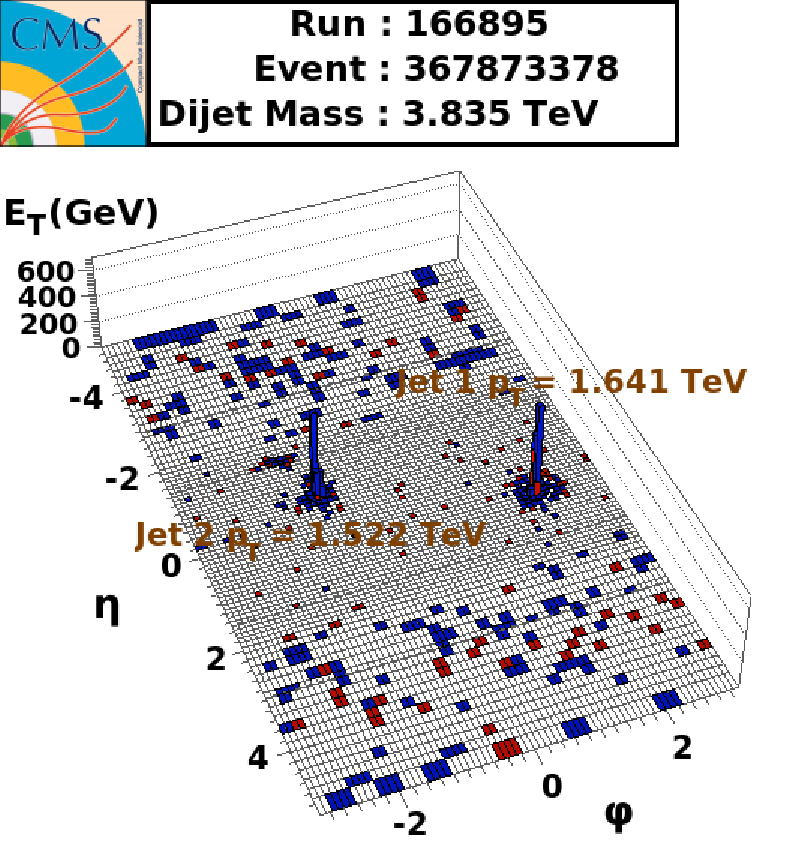
\includegraphics[width=0.37\textwidth]{Figures/EventDisplay_1st_lego.pdf}
    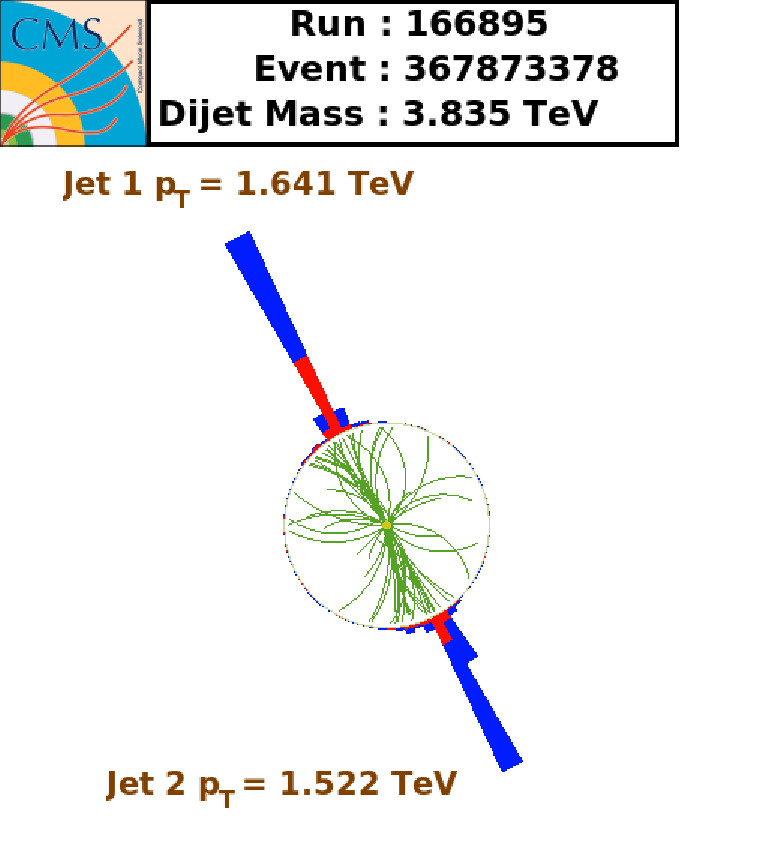
\includegraphics[width=0.37\textwidth]{Figures/EventDisplay_1st_rhophi.pdf}
    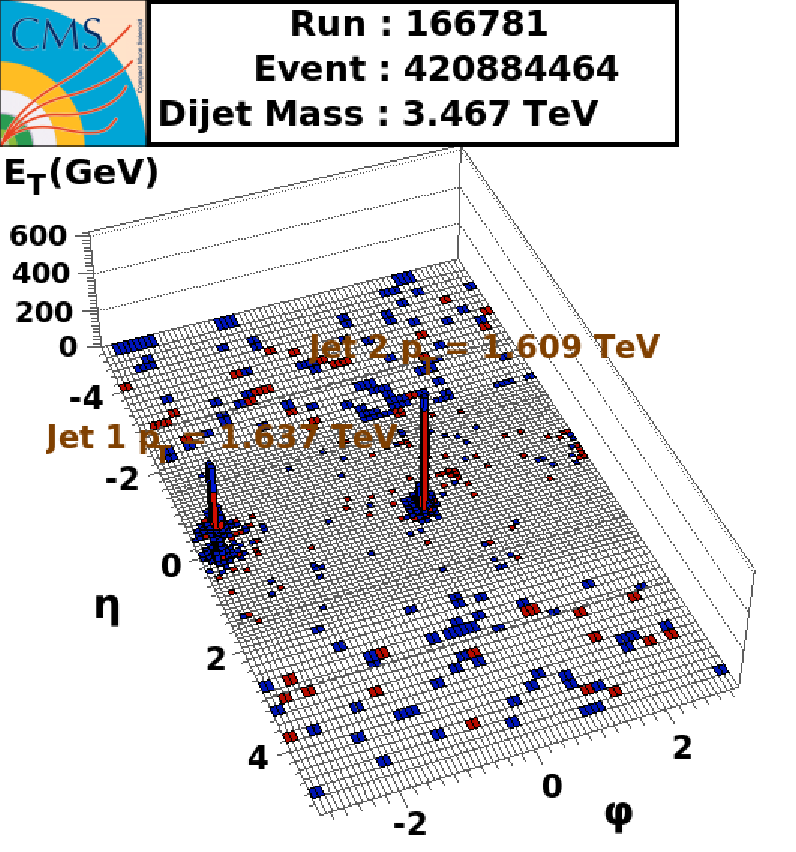
\includegraphics[width=0.37\textwidth]{Figures/EventDisplay_2nd_lego.pdf}
    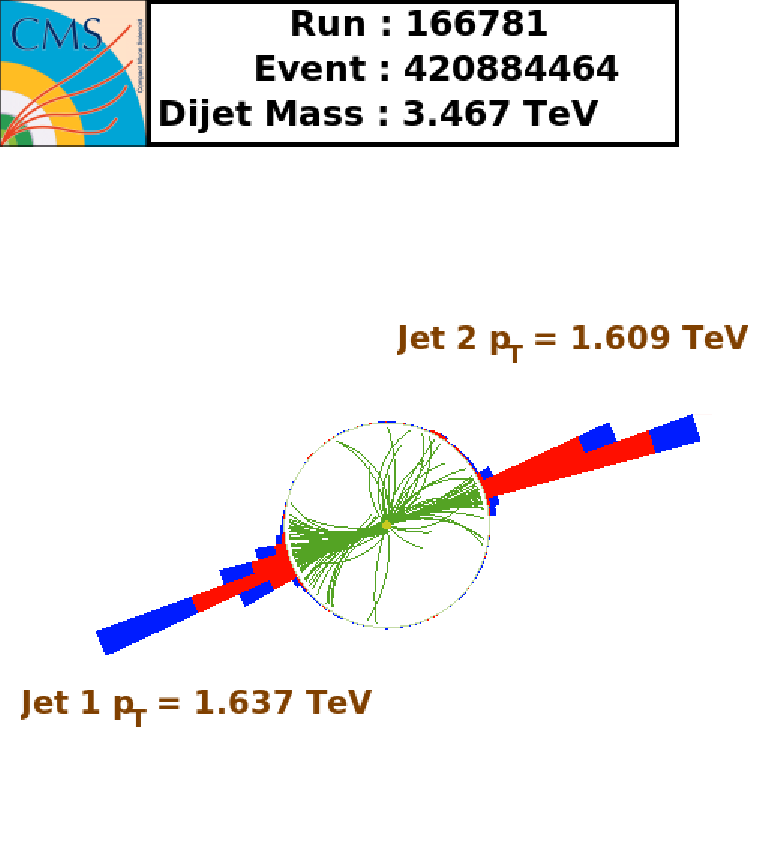
\includegraphics[width=0.37\textwidth]{Figures/EventDisplay_2nd_rhophi.pdf}
    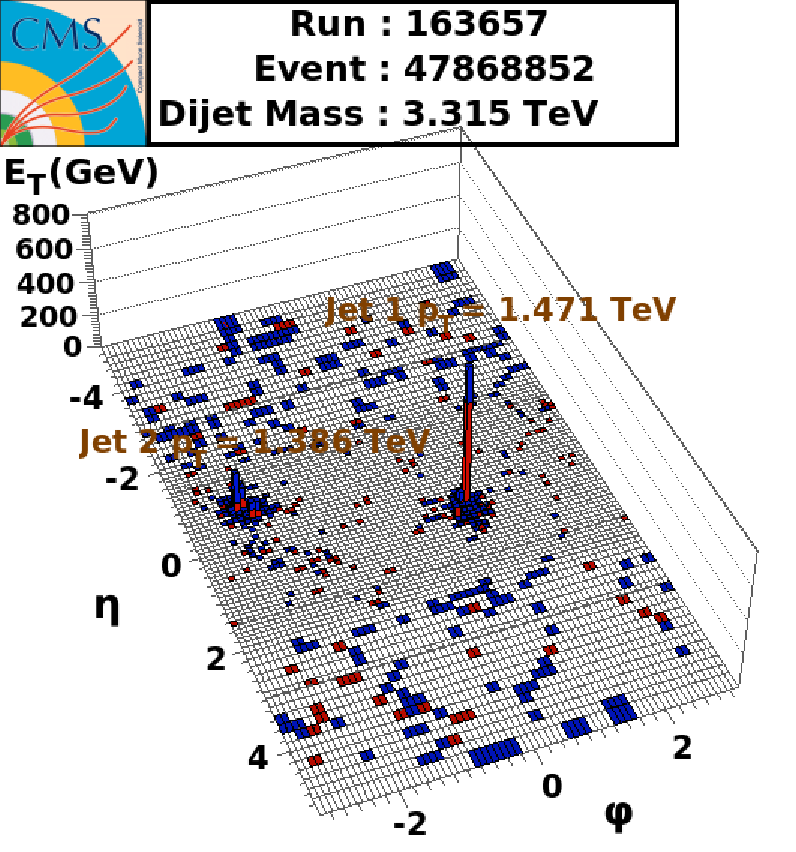
\includegraphics[width=0.37\textwidth]{Figures/EventDisplay_3rd_lego.pdf}
    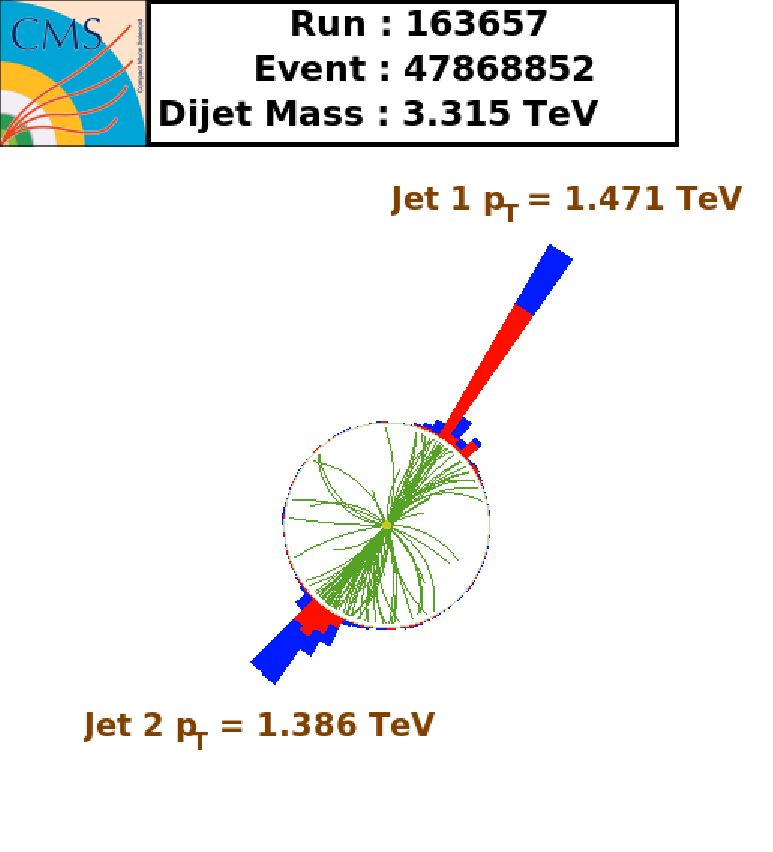
\includegraphics[width=0.37\textwidth]{Figures/EventDisplay_3rd_rhophi.pdf}
    \caption{Lego (left) and $\rho-\phi$ (right) displays of the 1st to 3rd Highest Masss Dijet Events}
    \label{MultiEventDisplay1}
  \end{center}
\end{figure}

\clearpage

\begin{figure}[!ht]
  \begin{center}
    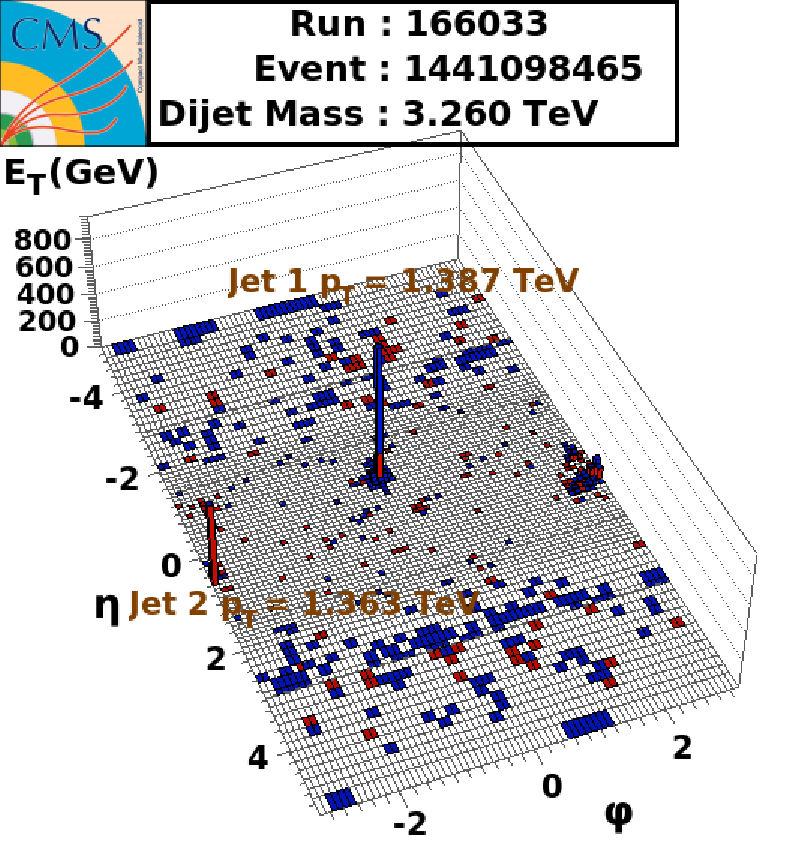
\includegraphics[width=0.37\textwidth]{Figures/EventDisplay_4th_lego.pdf}
    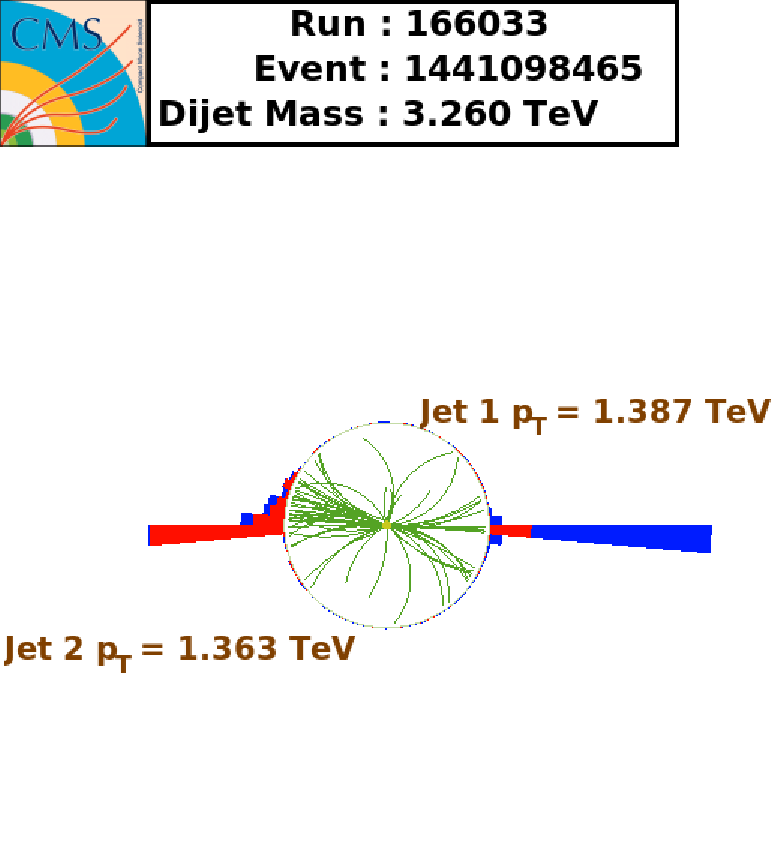
\includegraphics[width=0.37\textwidth]{Figures/EventDisplay_4th_rhophi.pdf}
    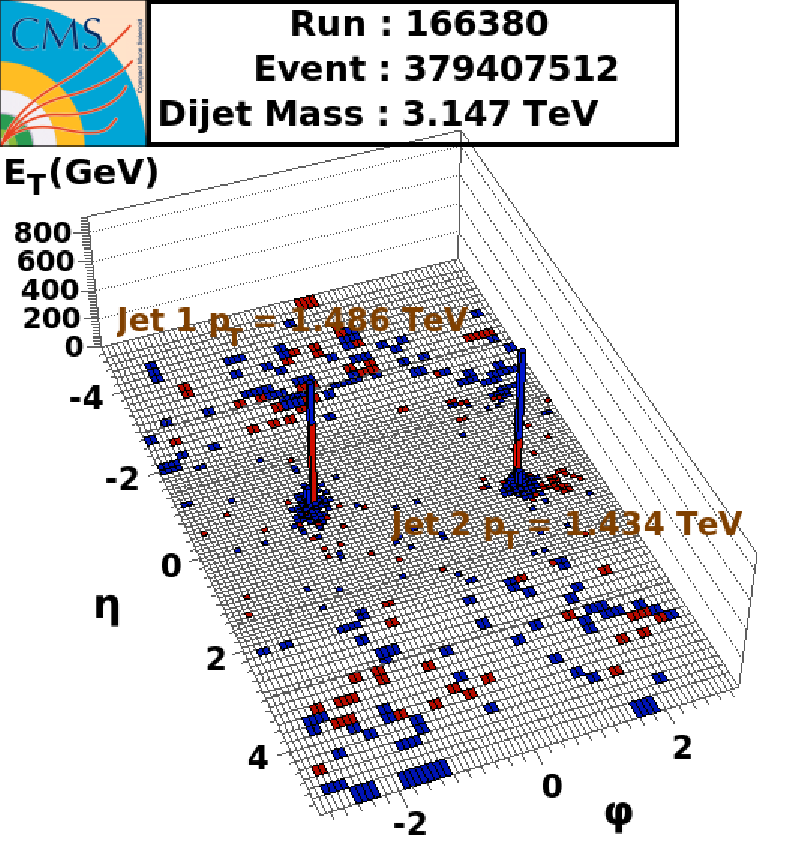
\includegraphics[width=0.37\textwidth]{Figures/EventDisplay_5th_lego.pdf}
    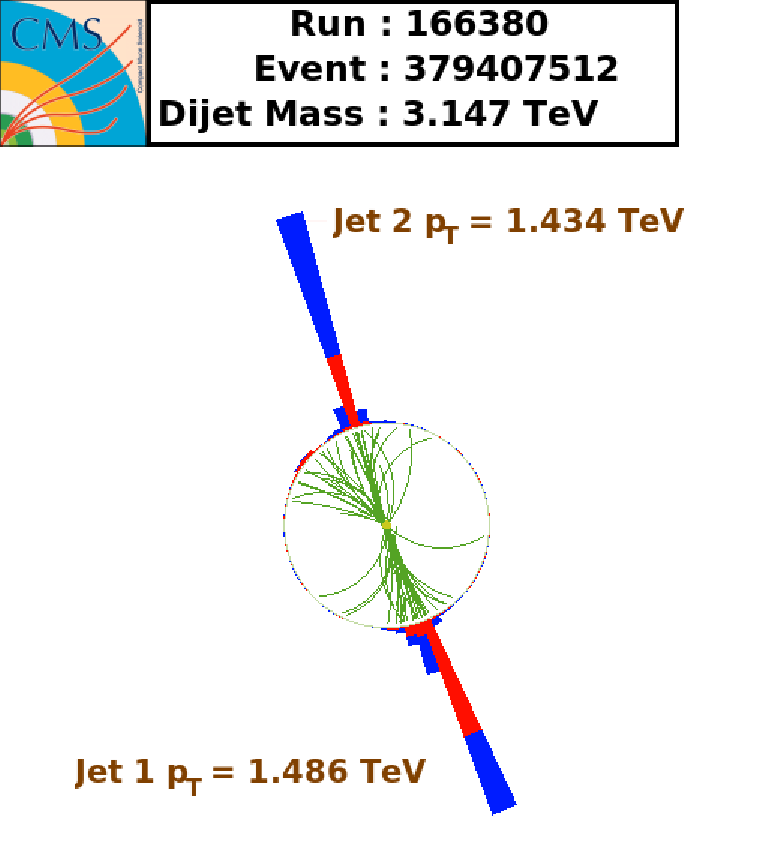
\includegraphics[width=0.37\textwidth]{Figures/EventDisplay_5th_rhophi.pdf}
    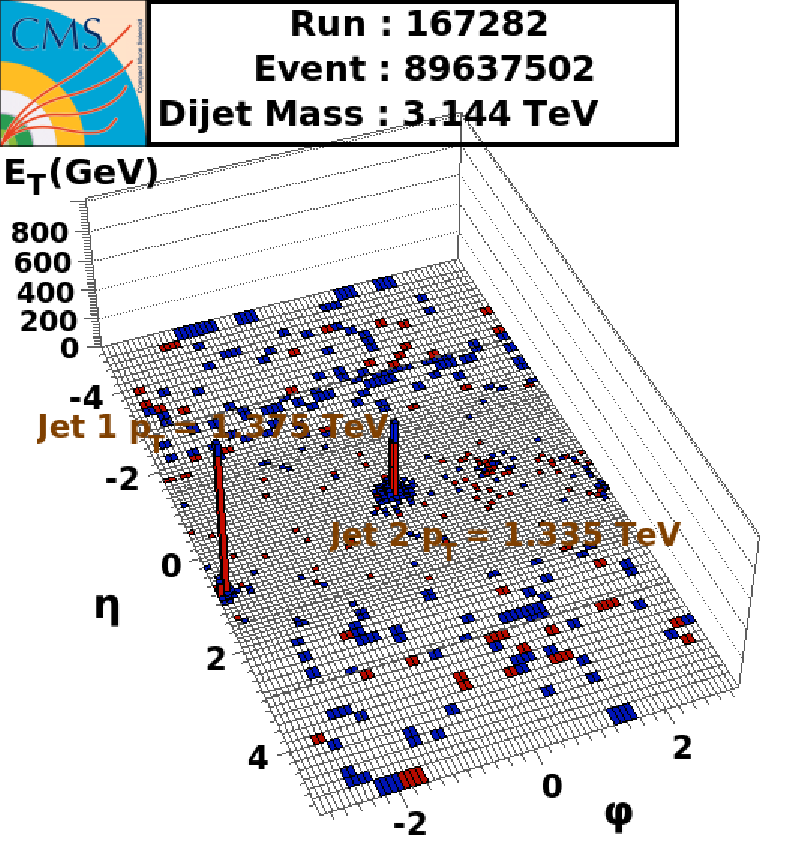
\includegraphics[width=0.37\textwidth]{Figures/EventDisplay_6th_lego.pdf}
    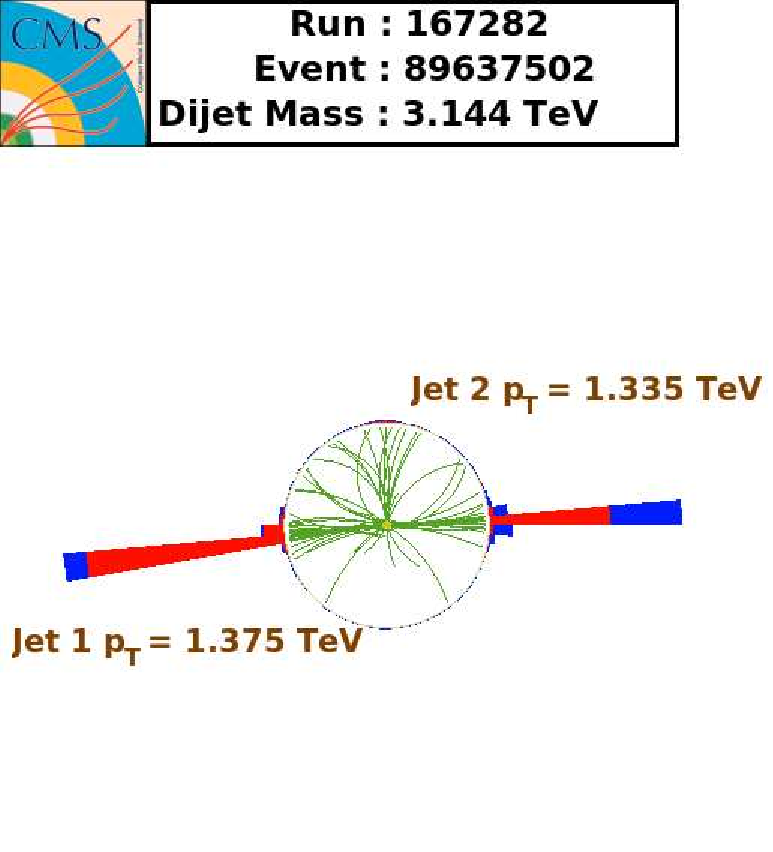
\includegraphics[width=0.37\textwidth]{Figures/EventDisplay_6th_rhophi.pdf}
    \caption{Lego (left) and $\rho-\phi$ (right) displays of the 4th to 6th Highest Masss Dijet Events}
    \label{MultiEventDisplay2}
  \end{center}
\end{figure}

\clearpage

\begin{figure}[!ht]
  \begin{center}
    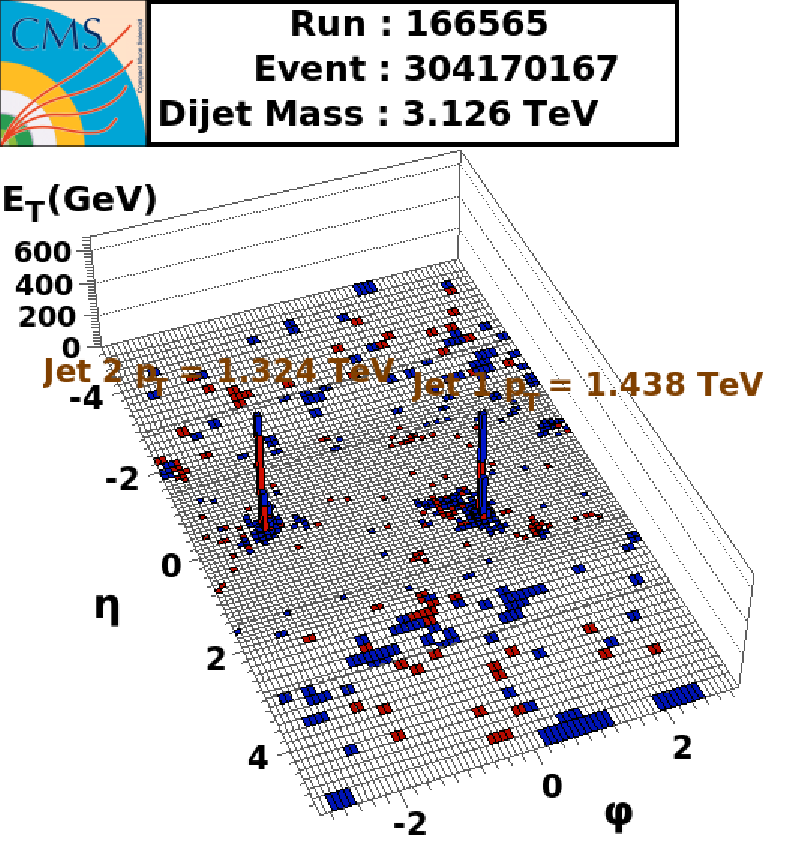
\includegraphics[width=0.30\textwidth]{Figures/EventDisplay_7th_lego.pdf}
    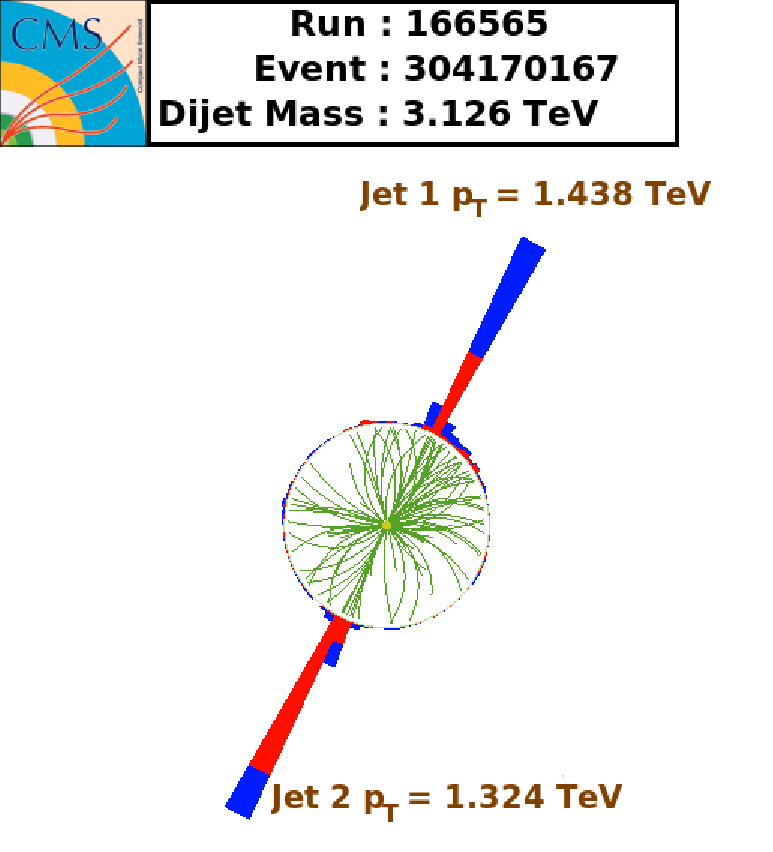
\includegraphics[width=0.30\textwidth]{Figures/EventDisplay_7th_rhophi.pdf}\\
    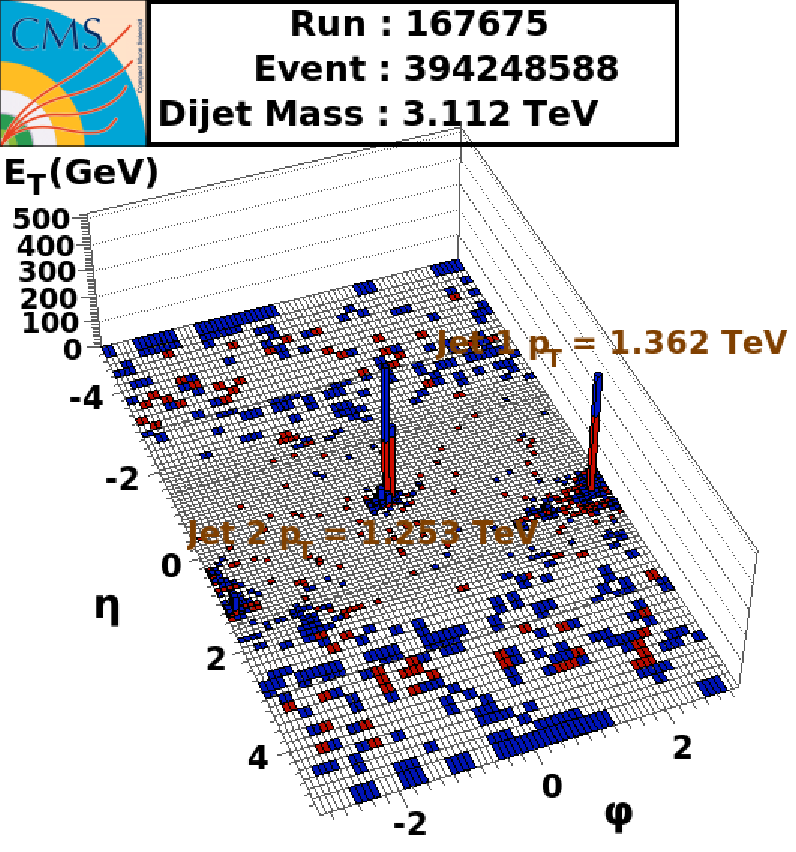
\includegraphics[width=0.30\textwidth]{Figures/EventDisplay_8th_lego.pdf}
    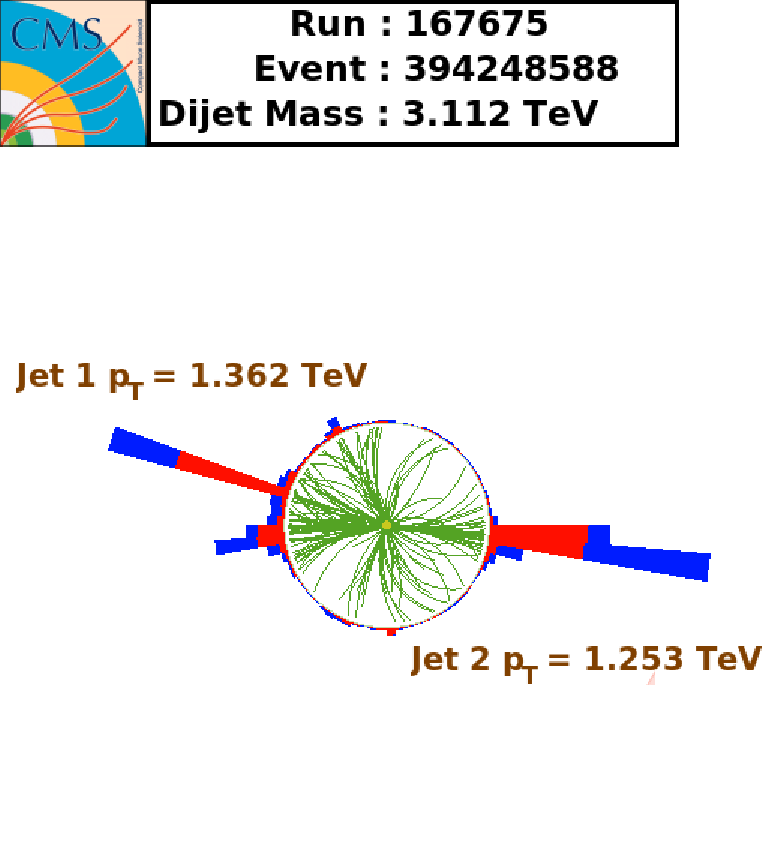
\includegraphics[width=0.30\textwidth]{Figures/EventDisplay_8th_rhophi.pdf}\\
    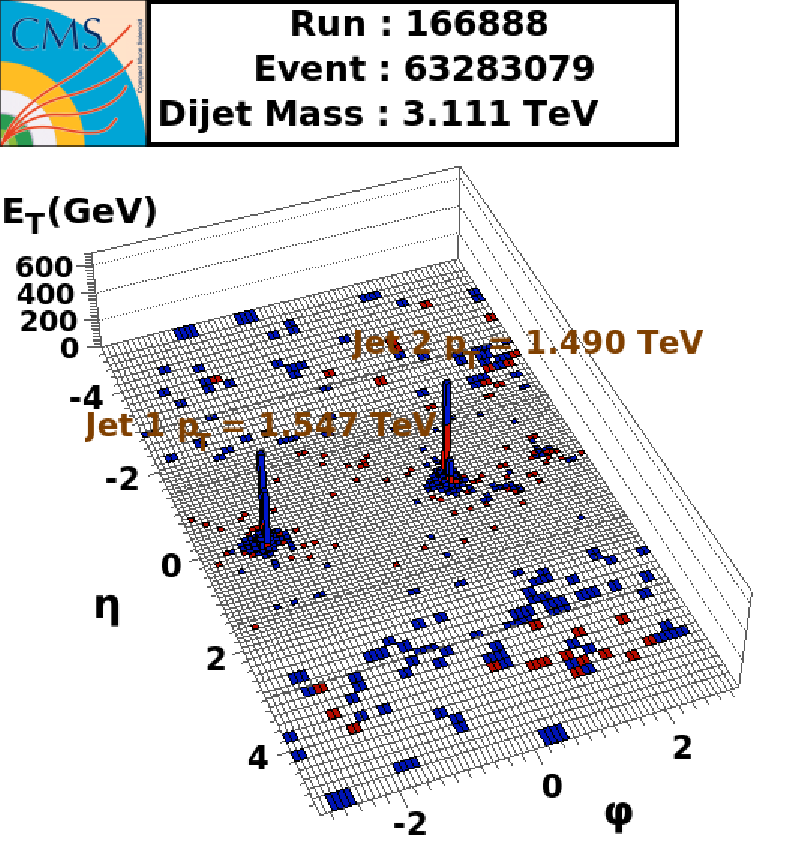
\includegraphics[width=0.30\textwidth]{Figures/EventDisplay_9th_lego.pdf}
    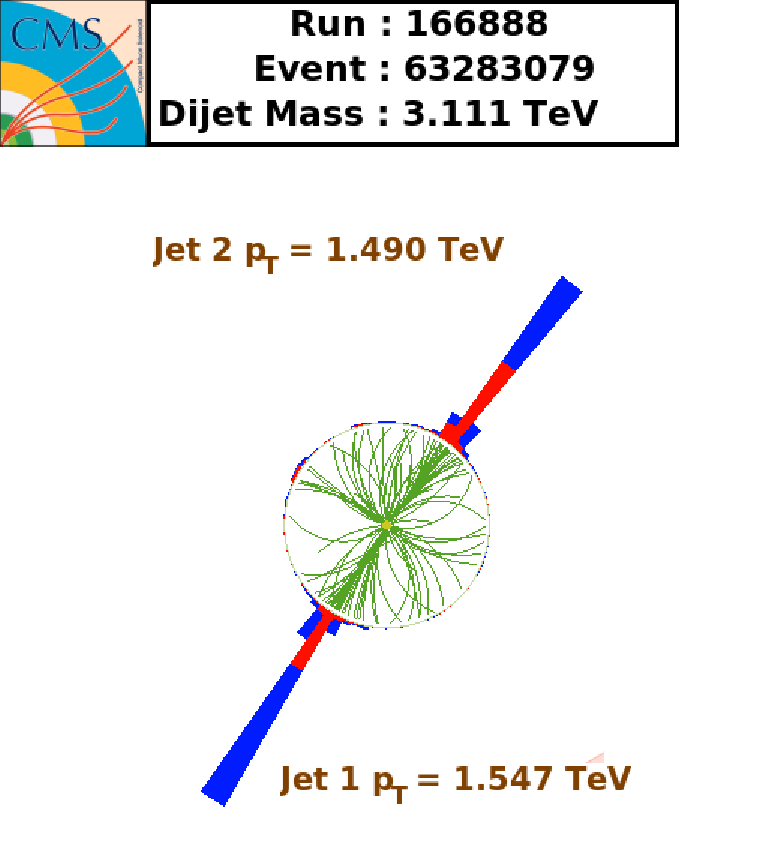
\includegraphics[width=0.30\textwidth]{Figures/EventDisplay_9th_rhophi.pdf}\\
    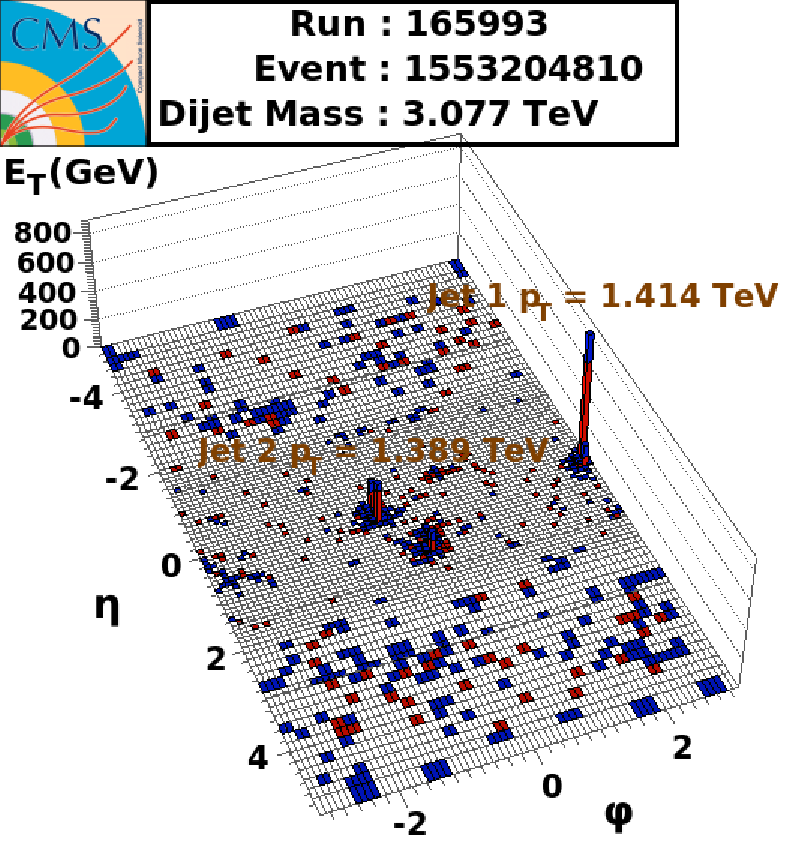
\includegraphics[width=0.30\textwidth]{Figures/EventDisplay_10th_lego.pdf}
    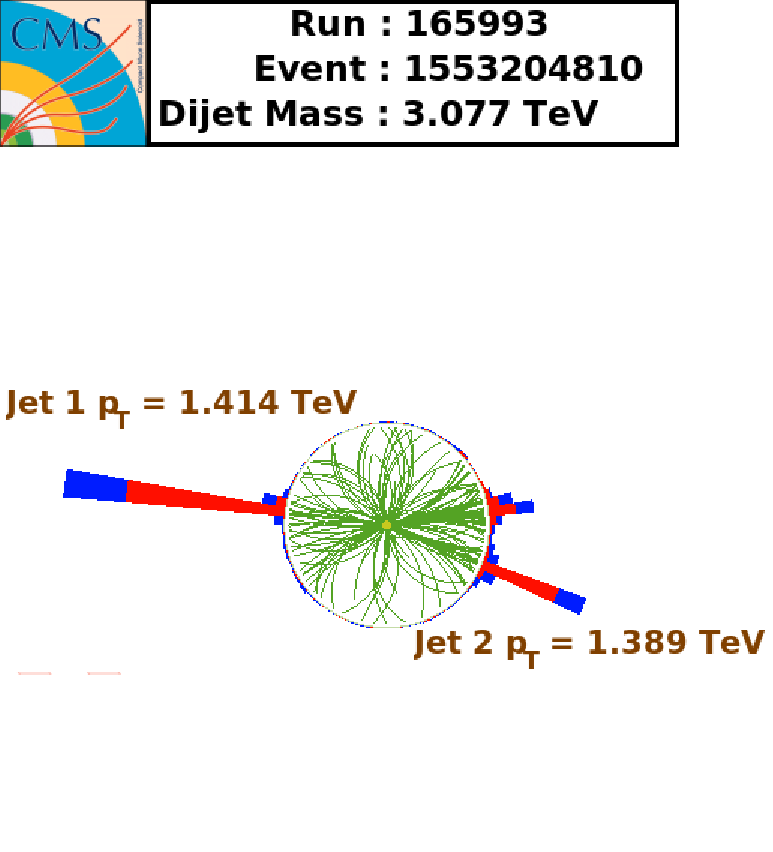
\includegraphics[width=0.30\textwidth]{Figures/EventDisplay_10th_rhophi.pdf}
    \caption{Lego (left) and $\rho-\phi$ (right) displays of the 7th to 10th Highest Masss Dijet Events}
    \label{MultiEventDisplay3}
  \end{center}
\end{figure}

\clearpage

\begin{table}[thb]
\centering
       \begin{tabular}{ |c|c||c|c|c|c|c|c|c|c| }
        \hline
        \multirow{2}{*}{$Run$} & \multirow{2}{*}{$Event$} & Dijet & $Jet$ 1   & $Jet$ 1 & $Jet$ 1  & $Jet$ 2 & $Jet$ 2 & $Jet$ 2 &  MET/$\Sigma E_T$\\
         & & Mass & Cor $p_T $ & $\eta$ & $\phi$  & Cor $p_T$ & $\eta$ & $\phi$ &  \\

          & & (TeV) & (TeV)  &  &  & (TeV) &  & &  \\
	\hline
	\hline
	166895 & 367873378 & 3.835 & 1.641 & 0.54 & 2.05 & 1.522 & -0.71 & -1.10 & 0.04 \\
	\hline
	166781 & 420884464 & 3.467 & 1.637 & -0.31 & -2.77 & 1.609 & 0.26 & 0.37 & 0.01\\
	\hline
	163657 & 47868852 & 3.315 & 1.471 & 0.35 & 0.97 & 1.386 & -0.69 & -2.23 & 0.03 \\
	\hline
	166033 & 1441098465 & 3.260 & 1.387 & -0.65 & -0.05 & 1.363 & 0.51 & 3.08 & 0.01 \\
	\hline
	166380 & 379407512 & 3.147 & 1.486 & -0.49 & -1.22 & 1.434 & 0.24 & 1.92 & 0.00 \\
	\hline
	166565 & 304170167 & 3.126 & 1.438 & 0.68 & 1.07 & 1.324 & -0.27 & -2.02 & 0.03 \\
	\hline
	167282 & 89637502 & 3.144 & 1.375 & 0.82 & -3.03 & 1.335 & -0.29 & 0.04 & 0.01 \\
	\hline
	167675 & 394248588 & 3.112 & 1.362 & 0.96 & 2.93 & 1.253 & -0.13 & -0.14 & 0.02 \\
	\hline
	166888 & 63283079 & 3.111 & 1.547 & 0.11 & -2.14 & 1.490 & -0.21 & 0.94 & 0.02 \\
	\hline
	165993 & 1553204810 & 3.077 & 1.414 & 0.16 & 3.01 & 1.389 & 0.51 & -0.16 & 0.01 \\
	\hline
       \end{tabular}
       \caption{Dijet properties for 10 highest mass events for calojet (Leading jets corrected $p_T$, $\eta$, $\phi$, 
	 corrected Dijet Mass, and Missing ET/Sum ET).}
       \label{table_highmass2}
\end{table}
      
%\vspace*{1in}
%\begin{table}[tbh]
%\centering
%       \begin{tabular}{ |c|c||c|c|c| }
%        \hline
%        \multirow{2}{*}{$Run$} & \multirow{2}{*}{$Event$} & $Jet$ 1  & $Jet$ 2 & Dijet Mass \\
%         & & PF Cor $p_T$  & PF Cor $p_T$ & from PFJets \\
%         & & (GeV) & (GeV) & (GeV) \\
%       \hline
%        \hline
%	138919 & 32253996  & 539 & 516 & 1941 \\
%        \hline
%	139370 & 132046118 & 457 & 447 & 1374 \\
%	\hline
%	139368 & 25590516  & 610 & 609 & 1267 \\
%	\hline
%	139370 & 403257286 & 421 & 384 & 1065 \\
%	\hline
%	138921 & 16936769  & 284 & 258 & 1040 \\
%	\hline
%	139096 & 247776848 & 361 & 319 & 976 \\
%	\hline
%	139347 & 252029032 & 334 & 299 & 915 \\
%        \hline
%	139370 & 511769839 & 289 & 294 & 904 \\
%	\hline
%	139365 & 65727014  & 339 & 324 & 868 \\
%	\hline
%	138737 & 44851731  & 418 & 385 & 855 \\
%        \hline
%        \end{tabular}
%        \caption{Particle Flow Corrected $p_T$ and dijet mass of leading PF Jets matched to CaloJets for the 
%	same events as in table~\ref{table_highmass2}.  Jet 1 and 2 in this table are matched 
%	to Jet 1 and 2 in table~\ref{table_highmass2} using $\Delta R$. Note: table for the 10 highest mass 
%	dijet events in a slighly older sample, so it needs updating, but the first 4 events in this 
%	table are also in the above table and those events can be compared. }
%        \label{table_highmass3}
%\end{table}



\clearpage
